\documentclass[12pt]{article}

% Packages
\usepackage{amsmath, amsthm, amssymb, amsfonts}
\usepackage{mathtools}
\usepackage{tikz}
\usepackage{geometry}                            % To adjust margins
\usepackage{enumitem}                            % For custom lists
\usepackage{hyperref}                            % For hyperlinks
\geometry{a4paper, margin=0.8in}                   % Set page margins
\usepackage{listings}
\usepackage{xcolor}
\usepackage{graphicx} % Add this to your preamble if not already included
\usepackage{float} % Include this in the preamble for the 'H' float option



\lstset{
    basicstyle=\ttfamily\footnotesize,
    keywordstyle=\color{blue}\bfseries,
    stringstyle=\color{red},
    commentstyle=\color{green!70!black},
    numbers=left,
    numberstyle=\tiny\color{gray},
    breaklines=true,
    frame=single,
    captionpos=b,
    tabsize=2
}

\DeclarePairedDelimiter\floor{\lfloor}{\rfloor}

% Theorem, Lemma, Corollary, and Proof Environments
\newtheorem{theorem}{Theorem}[section]
\newtheorem{lemma}[theorem]{Lemma}
\newtheorem{corollary}[theorem]{Corollary}

% Definition and Remark
\theoremstyle{definition}
\newtheorem{definition}[theorem]{Definition}
\newtheorem{example}[theorem]{Example}
\newtheorem{remark}[theorem]{Remark}
\newtheorem{proposition}[theorem]{Proposition}

% Title, Author, and Date
\title{An overview of parallelization techniques on Fast Fourier Transformation}
\author{Mircea Măierean, Robert-Petrișor Manea, Andreea-Selena Lung}
\date{\today}

% Document Begin
\begin{document}

\maketitle

% Abstract
\begin{abstract}
This paper presents different techniques for parallelizing the Fast Fourier Transformation algorithm. These techniques are applied in the multiplication of two polynomials, gradually improving each iteration with different approaches.
\end{abstract}

% Table of Contents (optional)
\tableofcontents


% Introduction
\section{Brief History}

In this paper, we will analyze an algorithm that allows us to multiply two polynomials of length $n$ in $O(n \log n)$ time, which is better than the trivial multiplication that takes $O(n^2)$ time, or Karatsuba's proposed idea that runs in $O(n^ {\log 3})$.

The discovery of the \textbf{Fast Fourier Transformation (FFT)} is attributed to Cooley and Tukey, who published an algorithm in 1965, but, in fact, the FFT has been discovered repeatedly before, although the importance of it was not understood before the inventions of modern computers.

Some researchers attribute the discovery of the FFT to Runge and König in 1924, but actually Gauss developed such a method already in 1805, but never published it.

\section{Discrete Fourier Transform}

Let there be a polynomial of degree \( n - 1 \): 
\[
A(x) = a_0 x^0 + a_1 x^1 + \dots + a_{n-1} x^{n-1}
\]

Without loss of generality, we assume that \( n \) — the number of coefficients — is a power of \( 2 \). If \( n \) is not a power of \( 2 \), then we simply add the missing terms \( a_i x^i \) and set the coefficients \( a_i \) to \( 0 \).

The theory of complex numbers tells us that the equation \( x^n = 1 \) has \( n \) complex solutions (called the \( n \)-th roots of unity), and the solutions are of the form \( w_{n, k} = e^{\frac{2 k \pi i}{n}} \) with \( k = 0 \dots n-1 \). Additionally, these complex numbers have some very interesting properties:
e.g., the principal \( n \)-th root \( w_n = w_{n, 1} = e^{\frac{2 \pi i}{n}} \) can be used to describe all other \( n \)-th roots: \( w_{n, k} = (w_n)^k \).

\begin{figure}[h!]
\centering
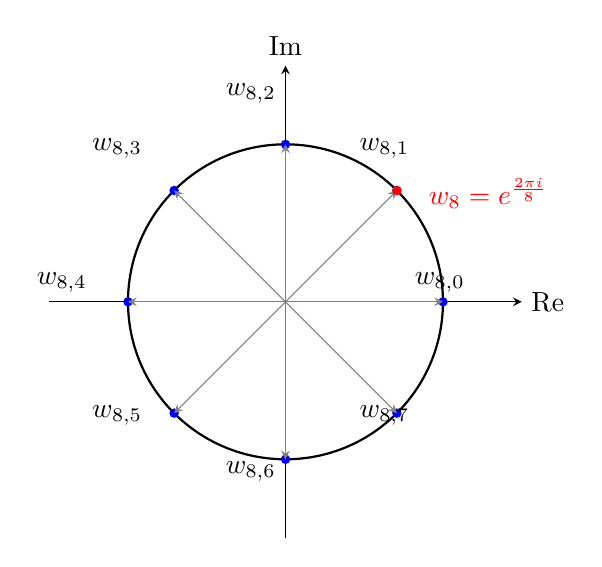
\begin{tikzpicture}[scale=2, >=stealth]
    % Draw the circle
    \draw[thick] (0,0) circle(1);

    % Draw the axes
    \draw[->] (-1.5,0) -- (1.5,0) node[anchor=west] {Re};
    \draw[->] (0,-1.5) -- (0,1.5) node[anchor=south] {Im};

    % Define the number of roots
    \def\n{8}

    % Draw the roots of unity
    \foreach \k in {0,...,7} {
        \coordinate (W\k) at ({cos(360*\k/\n)}, {sin(360*\k/\n)});
        \fill[blue] (W\k) circle(0.03); % Draw the points
        \draw[->, thin, gray] (0,0) -- (W\k); % Draw radius lines
        \node[anchor=south east] at ({1.2*cos(360*\k/\n)}, {1.2*sin(360*\k/\n)}) 
            {$w_{\n,\k}$}; % Label the points
    }
    
    % Highlight the principal root
    \fill[red] ({cos(360*1/\n)}, {sin(360*1/\n)}) circle(0.03); 
    \node[anchor=north west, red] at ({1.2*cos(360*1/\n)}, {1.2*sin(360*1/\n)}) 
        {$w_\n = e^{\frac{2\pi i}{\n}}$};

\end{tikzpicture}
\caption{The unit circle in the complex plane with 8 roots of unity.}
\label{fig:unit-circle}
\end{figure}

The \textbf{Discrete Fourier transform (DFT)} of the polynomial $A(x)$ (or equivalently the vector of coefficients $(a_0, a_1, \dots, a_{n-1})$ is defined as the values of the polynomial at the points $x = w_{n, k}$, i.e. it is the vector:


\begin{align}
\text{DFT}(a_0, a_1, \dots, a_{n-1}) &= (y_0, y_1, \dots, y_{n-1}) \\
&= (A(w_{n, 0}), A(w_{n, 1}), \dots, A(w_{n, n-1})) \\
&= (A(w_n^0), A(w_n^1), \dots, A(w_n^{n-1}))
\end{align}

Similarly the \textbf{Inverse Discrete Fourier Transform} is defined:
The $inverse DFT$ of values of the polynomial $(y_0, y_1, \dots, y_{n-1})$ are the coefficients of the polynomial $(a_0, a_1, \dots, a_{n-1})$.

$$\text{InverseDFT}(y_0, y_1, \dots, y_{n-1}) = (a_0, a_1, \dots, a_{n-1})$$

Thus, if a direct DFT computes the values of the polynomial at the points at the $n$-th roots, the inverse DFT can restore the coefficients of the polynomial using those values.



% Preliminaries or Notation (optional)
\section{Application: Fast Multiplication of Polynomials}

Let there be two polynomials $A$ and $B$.
We compute the DFT for each of them: $\text{DFT}(A)$ and $\text{DFT}(B)$.

What happens if we multiply these polynomials? Obviously at each point the values are simply multiplied, i.e.

$$(A \cdot B)(x) = A(x) \cdot B(x).$$

This means that if we multiply the vectors $\text{DFT}(A)$ and $\text{DFT}(B)$ - by multiplying each element of one vector by the corresponding element of the other vector - then we get nothing other than the DFT of the polynomial $\text{DFT}(A \cdot B)$:

$$\text{DFT}(A \cdot B) = \text{DFT}(A) \cdot \text{DFT}(B)$$

Finally, applying the inverse DFT, we obtain:

$$A \cdot B = \text{InverseDFT}(\text{DFT}(A) \cdot \text{DFT}(B))$$

On the right the product of the two DFTs we mean the pairwise product of the vector elements.
This can be computed in $O(n)$ time.
If we can compute the DFT and the inverse DFT in $O(n \log n)$, then we can compute the product of the two polynomials (and consequently also two long numbers) with the same time complexity.

It should be noted, that the two polynomials should have the same degree.
Otherwise the two result vectors of the DFT have different length.
We can accomplish this by adding coefficients with the value $0$.

And also, since the result of the product of two polynomials is a polynomial of degree $2 (n - 1)$, we have to double the degrees of each polynomial (again by padding $0$s).
From a vector with $n$ values we cannot reconstruct the desired polynomial with $2n - 1$ coefficients.


\section{Fast Fourier Transform}

The \textbf{Fast Fourier Transform} is a method that allows computing the DFT in $O(n \log n)$ time. The basic idea of the FFT is to apply divide and conquer.

We divide the coefficient vector of the polynomial into two vectors, recursively compute the DFT for each of them, and combine the results to compute the DFT of the complete polynomial.

So let there be a polynomial $A(x)$ with degree $n - 1$, where $n$ is a power of $2$, and $n > 1$:

$$A(x) = a_0 x^0 + a_1 x^1 + \dots + a_{n-1} x^{n-1}$$

We divide it into two smaller polynomials, the one containing only the coefficients of the even positions, and the one containing the coefficients of the odd positions:

\begin{align}
A_0(x) &= a_0 x^0 + a_2 x^1 + \dots + a_{n-2} x^{\frac{n}{2}-1} \\
A_1(x) &= a_1 x^0 + a_3 x^1 + \dots + a_{n-1} x^{\frac{n}{2}-1}
\end{align}


It is easy to see that

$$A(x) = A_0(x^2) + x A_1(x^2).$$

The polynomials $A_0$ and $A_1$ have only half as many coefficients as the polynomial $A$.
If we can compute the $\text{DFT}(A)$ in linear time using $\text{DFT}(A_0)$ and $\text{DFT}(A_1)$, then we get the recurrence $T_{\text{DFT}}(n) = 2 T_{\text{DFT}}\left(\frac{n}{2}\right) + O(n)$ for the time complexity, which results in $T_{\text{DFT}}(n) = O(n \log n)$.


Let's learn how we can accomplish that.

Suppose we have computed the vectors $\left(y_k^0\right)_{k=0}^{n/2-1} = \text{DFT}(A_0)$ and $\left(y_k^1\right)_{k=0}^{n/2-1} = \text{DFT}(A_1)$.
Let us find a expression for $\left(y_k\right)_{k=0}^{n-1} = \text{DFT}(A)$.

For the first $\frac{n}{2}$ values we can just use the previously noted equation $A(x) = A_0(x^2) + x A_1(x^2)$:

$$y_k = y_k^0 + w_n^k y_k^1, \quad k = 0 \dots \frac{n}{2} - 1.$$

However for the second $\frac{n}{2}$ values we need to find a slightly, different expression:

\begin{align}
y_{k+n/2} &= A\left(w_n^{k+n/2}\right) \\
&= A_0\left(w_n^{2k+n}\right) + w_n^{k + n/2} A_1\left(w_n^{2k+n}\right) \\
&= A_0\left(w_n^{2k} w_n^n\right) + w_n^k w_n^{n/2} A_1\left(w_n^{2k} w_n^n\right) \\
&= A_0\left(w_n^{2k}\right) - w_n^k A_1\left(w_n^{2k}\right) \\
&= y_k^0 - w_n^k y_k^1
\end{align}

Here we used again $A(x) = A_0(x^2) + x A_1(x^2)$ and the two identities $w_n^n = 1$ and $w_n^{n/2} = -1$.

Therefore we get the desired formulas for computing the whole vector $(y_k)$:

\begin{align}
y_k &= y_k^0 + w_n^k y_k^1, &\quad k = 0 \dots \frac{n}{2} - 1, \\
y_{k+n/2} &= y_k^0 - w_n^k y_k^1, &\quad k = 0 \dots \frac{n}{2} - 1.
\end{align}


This pattern $a + b$ and $a - b$ is sometimes called a \textbf{butterfly}, that will be discussed later


\section{Inverse FFT}

Let the vector $(y_0, y_1, \dots y_{n-1})$ - the values of polynomial $A$ of degree $n - 1$ in the points $x = w_n^k$ - be given.
We want to restore the coefficients $(a_0, a_1, \dots, a_{n-1})$ of the polynomial.
This known problem is called \textbf{interpolation}, and there are general algorithms for solving it.
But in this special case (since we know the values of the points at the roots of unity), we can obtains a much simpler algorithm (that is practically the same as the direct FFT).

We can write the DFT, according to its definition, in the matrix form:

\begin{align}
\begin{pmatrix}
w_n^0 & w_n^0 & w_n^0 & w_n^0 & \cdots & w_n^0 \\
w_n^0 & w_n^1 & w_n^2 & w_n^3 & \cdots & w_n^{n-1} \\
w_n^0 & w_n^2 & w_n^4 & w_n^6 & \cdots & w_n^{2(n-1)} \\
w_n^0 & w_n^3 & w_n^6 & w_n^9 & \cdots & w_n^{3(n-1)} \\
\vdots & \vdots & \vdots & \vdots & \ddots & \vdots \\
w_n^0 & w_n^{n-1} & w_n^{2(n-1)} & w_n^{3(n-1)} & \cdots & w_n^{(n-1)(n-1)}
\end{pmatrix} \begin{pmatrix}
a_0 \\ a_1 \\ a_2 \\ a_3 \\ \vdots \\ a_{n-1}
\end{pmatrix} = \begin{pmatrix}
y_0 \\ y_1 \\ y_2 \\ y_3 \\ \vdots \\ y_{n-1}
\end{pmatrix}
\end{align}

Thus we can compute the vector $(a_0, a_1, \dots, a_{n-1})$ by multiplying the vector $(y_0, y_1, \dots y_{n-1})$ from the left with the inverse of the matrix:

\begin{align}
\begin{pmatrix}
a_0 \\ a_1 \\ a_2 \\ a_3 \\ \vdots \\ a_{n-1}
\end{pmatrix} = \begin{pmatrix}
w_n^0 & w_n^0 & w_n^0 & w_n^0 & \cdots & w_n^0 \\
w_n^0 & w_n^1 & w_n^2 & w_n^3 & \cdots & w_n^{n-1} \\
w_n^0 & w_n^2 & w_n^4 & w_n^6 & \cdots & w_n^{2(n-1)} \\
w_n^0 & w_n^3 & w_n^6 & w_n^9 & \cdots & w_n^{3(n-1)} \\
\vdots & \vdots & \vdots & \vdots & \ddots & \vdots \\
w_n^0 & w_n^{n-1} & w_n^{2(n-1)} & w_n^{3(n-1)} & \cdots & w_n^{(n-1)(n-1)}
\end{pmatrix}^{-1} \begin{pmatrix}
y_0 \\ y_1 \\ y_2 \\ y_3 \\ \vdots \\ y_{n-1}
\end{pmatrix}
\end{align}


A quick check can verify that the inverse of the matrix has the following form:

\begin{align}
\frac{1}{n}
\begin{pmatrix}
w_n^0 & w_n^0 & w_n^0 & w_n^0 & \cdots & w_n^0 \\
w_n^0 & w_n^{-1} & w_n^{-2} & w_n^{-3} & \cdots & w_n^{-(n-1)} \\
w_n^0 & w_n^{-2} & w_n^{-4} & w_n^{-6} & \cdots & w_n^{-2(n-1)} \\
w_n^0 & w_n^{-3} & w_n^{-6} & w_n^{-9} & \cdots & w_n^{-3(n-1)} \\
\vdots & \vdots & \vdots & \vdots & \ddots & \vdots \\
w_n^0 & w_n^{-(n-1)} & w_n^{-2(n-1)} & w_n^{-3(n-1)} & \cdots & w_n^{-(n-1)(n-1)}
\end{pmatrix}
\end{align}

Thus we obtain the formula:

$$a_k = \frac{1}{n} \sum_{j=0}^{n-1} y_j w_n^{-k j}$$

Comparing this to the formula for $y_k$

$$y_k = \sum_{j=0}^{n-1} a_j w_n^{k j},$$

we notice that these problems are almost the same, so the coefficients $a_k$ can be found by the same divide and conquer algorithm, as well as the direct FFT, only instead of $w_n^k$ we have to use $w_n^{-k}$, and at the end we need to divide the resulting coefficients by $n$.

Thus the computation of the inverse DFT is almost the same as the calculation of the direct DFT, and it also can be performed in $O(n \log n)$ time.

% Conclusion
\section{Sequential implementation}

Here we present a simple recursive implementation of the FFT and the inverse FFT, both in one function, since the difference between the forward and the inverse FFT are so minimal.
To store the complex numbers we use the complex type in the C++ STL.

\begin{lstlisting}[language=C++, caption={Recursive sequential implementation of the code.}]
const double pi = acos(-1);

void fft(vector<complex<double>> &p, bool inverse)
{
    int n = p.size();
    if (n == 1) return;
    vector<complex<double>> pe(n / 2), po(n / 2);
    for (int i = 0; 2 * i < n; ++i)
        pe[i] = p[2 * i], po[i] = p[2 * i + 1];
    fft(pe, inverse);
    fft(po, inverse);
    double theta = 2.00 * pi / n * (inverse ? -1 : 1);
    complex<double> w(1), wn(cos(theta), sin(theta));
    for (int i = 0; 2 * i < n; ++i)
    {
        // compute the pairs x and -x
        p[i] = pe[i] + w * po[i];
        p[i + n / 2] = pe[i] - w * po[i];
        if (inverse)
        {
            p[i] /= 2;
            p[i + n / 2] /= 2;
        }
        w *= wn;
    }
}
vector<long long> multiply(vector<long long> const &a, vector<long long> const &b)
{
    vector<complex<double>> fa(a.begin(), a.end()), fb(b.begin(), b.end());
    int polynomial_size = a.size() + b.size();
    int n = 1;

    while (n < a.size() + b.size())
        n <<= 1;

    fa.resize(n);
    fb.resize(n);

    fft(fa, false);
    fft(fb, false);
    for (int i = 0; i < n; i++)
        fa[i] *= fb[i];
    fft(fa, true);

    vector<long long> result(n);
    for (int i = 0; i < n; i++)
        result[i] = round(fa[i].real());

    while (result.size() >= polynomial_size)
        result.pop_back();

    return result;
}

\end{lstlisting}

The function gets passed a vector of coefficients, and the function will compute the DFT or inverse DFT and store the result again in this vector.

The argument $\text{invert}$ shows whether the direct or the inverse DFT should be computed.

Inside the function we first check if the length of the vector is equal to one, if this is the case then we don't have to do anything.

Otherwise we divide the vector $a$ into two vectors $a0$ and $a1$ and compute the DFT for both recursively.

Then we initialize the value $wn$ and a variable $w$, which will contain the current power of $wn$.

Then the values of the resulting DFT are computed using the above formulas.

If the flag $\text{invert}$ is set, then we replace $wn$ with $wn^{-1}$, and each of the values of the result is divided by $2$ (since this will be done in each level of the recursion, this will end up dividing the final values by $n$).

At the end, we clear the additional zeroes that have been padded, to ensure that the polynomials have the same size for their multiplication.

\section{Parallelized implementation}

As we have seen in the \text{fft} function, there are 2 recursive calls for the same function, that run independently, without any synchronization required between them. We can parallelize this computation, thus computing both of the required parts at the same time. As the number of process grow exponentially by this approach, we will set a maximum depth of the recursion, that can be adjusted depending on the hardware capacities of the computer. 
\begin{lstlisting}[language=C++, caption={Recursive parallelized implementation of the code.}]
const double pi = acos(-1);
int max_depth;

void fft(vector<complex<double>> &p, bool inverse, int depth = 0)
{
    int n = p.size();
    if (n == 1)
        return;

    vector<complex<double>> pe(n / 2), po(n / 2);
    for (int i = 0; i < n / 2; ++i)
    {
        pe[i] = p[2 * i];
        po[i] = p[2 * i + 1];
    }

    if (depth < max_depth)
    {
        auto future1 = async(fft, ref(pe), inverse, depth + 1);
        auto future2 = async(fft, ref(po), inverse, depth + 1);
        future1.get();
        future2.get();
    }
    else
    {
        fft(pe, inverse, depth + 1);
        fft(po, inverse, depth + 1);
    }

    double theta = 2.00 * pi / n * (inverse ? -1 : 1);
    complex<double> w(1), wn(cos(theta), sin(theta));
    for (int i = 0; i < n / 2; ++i)
    {
        p[i] = pe[i] + w * po[i];
        p[i + n / 2] = pe[i] - w * po[i];
        if (inverse)
        {
            p[i] /= 2;
            p[i + n / 2] /= 2;
        }
        w *= wn;
    }
}
\end{lstlisting}

% Conclusion
\section{Improved implementation: in-place computation}

To increase the efficiency we will switch from the recursive implementation to an iterative one. In the above recursive implementation we explicitly separated the vector $a$ into two vectors - the element on the even positions got assigned to one temporary vector, and the elements on odd positions to another.

However if we reorder the elements in a certain way, we don't need to create these temporary vectors (i.e. all the calculations can be done "in-place", right in the vector $A$ itself).

Note that at the first recursion level, the elements whose lowest bit of the position was zero got assigned to the vector $a_0$, and the ones with a one as the lowest bit of the position got assigned to $a_1$.

In the second recursion level the same thing happens, but with the second lowest bit instead, etc.

Therefore if we reverse the bits of the position of each coefficient, and sort them by these reversed values, we get the desired order (it is called the bit-reversal permutation).

For example the desired order for $n = 8$ has the form:

$$a = \bigg\{ \Big[ (a_0, a_4), (a_2, a_6) \Big], \Big[ (a_1, a_5), (a_3, a_7) \Big] \bigg\}$$

Indeed in the first recursion level (surrounded by curly braces), the vector gets divided into two parts $[a_0, a_2, a_4, a_6]$ and $[a_1, a_3, a_5, a_7]$.

As we see, in the bit-reversal permutation this corresponds to simply dividing the vector into two halves: the first $\frac{n}{2}$ elements and the last $\frac{n}{2}$ elements.
Then there is a recursive call for each halve.

Let the resulting DFT for each of them be returned in place of the elements themselves (i.e. the first half and the second half of the vector $a$ respectively.

$$a = \bigg\{ \Big[y_0^0, y_1^0, y_2^0, y_3^0\Big], \Big[y_0^1, y_1^1, y_2^1, y_3^1 \Big] \bigg\}$$

Now we want to combine the two DFTs into one for the complete vector.
The order of the elements is ideal, and we can also perform the union directly in this vector.

We can take the elements $y_0^0$ and $y_0^1$ and perform the butterfly transform.
The place of the resulting two values is the same as the place of the two initial values, so we get:

$$a = \bigg\{ \Big[y_0^0 + w_n^0 y_0^1, y_1^0, y_2^0, y_3^0\Big], \Big[y_0^0 - w_n^0 y_0^1, y_1^1, y_2^1, y_3^1\Big] \bigg\}$$


Similarly we can compute the butterfly transform of $y_1^0$ and $y_1^1$ and put the results in their place, and so on.
As a result we get:

$$a = \bigg\{ \Big[y_0^0 + w_n^0 y_0^1, y_1^0 + w_n^1 y_1^1, y_2^0 + w_n^2 y_2^1, y_3^0 + w_n^3 y_3^1\Big], \Big[y_0^0 - w_n^0 y_0^1, y_1^0 - w_n^1 y_1^1, y_2^0 - w_n^2 y_2^1, y_3^0 - w_n^3 y_3^1\Big] \bigg\}$$

\begin{lstlisting}[language=C++, caption={Iterative implementation of FFT.}]

const double PI = acos(-1);

void iterative_fft(vector<complex<double>> &p, bool inverse)
{
    int n = p.size();
    vector<complex<double>> temp(n);

    int log_n = log2(n);
    for (int i = 0; i < n; ++i)
    {
        int reversed = 0, x = i;
        for (int j = 0; j < log_n; ++j)
        {
            reversed = (reversed << 1) | (x & 1);
            x >>= 1;
        }
        if (i < reversed)
            swap(p[i], p[reversed]);
    }

    for (int len = 2; len <= n; len <<= 1)
    {
        double theta = 2.0 * PI / len * (inverse ? -1 : 1);
        complex<double> wn(cos(theta), sin(theta));
        for (int i = 0; i < n; i += len)
        {
            complex<double> w(1);
            for (int j = 0; j < len / 2; ++j)
            {
                complex<double> u = p[i + j];
                complex<double> v = w * p[i + j + len / 2];
                p[i + j] = u + v;
                p[i + j + len / 2] = u - v;
                w *= wn;
            }
        }
    }

    if (inverse)
    {
        for (auto &x : p)
            x /= n;
    }
}
\end{lstlisting}

% Conclusion
\section{MPI}
    
The root process (rank 0) reads the input polynomials and ensures their size is padded to the nearest power of two, a requirement for the FFT algorithm. The transformed coefficients of both polynomials are then broadcast to all processes, ensuring that every process has the necessary data for computation. Broadcasting simplifies communication, as all processes operate on the same set of data.

Each process performs point-wise multiplication on a distinct subset of the frequency-domain coefficients. This task is computationally independent, enabling efficient parallel execution without inter-process communication during this phase. The multiplication results are then sent back to the root process.

The root process gathers the modified coefficients and performs an inverse FFT to transform the product back to the time domain, resulting in the final polynomial coefficients. Any additional zero-padding is removed, and the trimmed result is written to an output file.

By distributing the point-wise multiplication and leveraging MPI's communication capabilities, the algorithm achieves significant performance improvements for large polynomial sizes. This parallel approach ensures scalability and efficient utilization of computational resources.

\begin{lstlisting}[language=C++, caption={FFT iterative parallelized implementation using MPI.}]
const double pi = acos(-1);

void fft(vector<complex<double>> &p, bool inverse)
{
    int n = p.size();
    if (n == 1)
        return;
    vector<complex<double>> pe(n / 2), po(n / 2);
    for (int i = 0; i < n / 2; ++i)
    {
        pe[i] = p[2 * i];
        po[i] = p[2 * i + 1];
    }

    fft(pe, inverse);
    fft(po, inverse);

    double theta = 2.00 * pi / n * (inverse ? -1 : 1);
    complex<double> w(1), wn(cos(theta), sin(theta));
    for (int i = 0; i < n / 2; ++i)
    {
        p[i] = pe[i] + w * po[i];
        p[i + n / 2] = pe[i] - w * po[i];
        if (inverse)
        {
            p[i] /= 2;
            p[i + n / 2] /= 2;
        }
        w *= wn;
    }
}

vector<long long> multiply(vector<long long> const &a, vector<long long> const &b, int rank, int size)
{
    vector<complex<double>> fa(a.begin(), a.end()), fb(b.begin(), b.end());
    int polynomial_size = a.size() + b.size(); // Store the expected size
    int n = 1;
    while (n < a.size() + b.size())
        n <<= 1;
    fa.resize(n);
    fb.resize(n);

    // Broadcast the input arrays to all processes
    if (rank == 0)
    {
        for (int i = 1; i < size; i++)
        {
            MPI_Send(fa.data(), n * 2, MPI_DOUBLE, i, 0, MPI_COMM_WORLD);
            MPI_Send(fb.data(), n * 2, MPI_DOUBLE, i, 1, MPI_COMM_WORLD);
        }
    }
    else
    {
        MPI_Recv(fa.data(), n * 2, MPI_DOUBLE, 0, 0, MPI_COMM_WORLD, MPI_STATUS_IGNORE);
        MPI_Recv(fb.data(), n * 2, MPI_DOUBLE, 0, 1, MPI_COMM_WORLD, MPI_STATUS_IGNORE);
    }

    // Perform FFT
    fft(fa, false);
    fft(fb, false);

    // Distribute multiplication work
    int chunk_size = n / size;
    int start = rank * chunk_size;
    int end = (rank == size - 1) ? n : (rank + 1) * chunk_size;

    // Perform multiplication for this process's chunk
    for (int i = start; i < end; i++)
        fa[i] *= fb[i];

    // Gather results back to process 0
    if (rank == 0)
    {
        for (int i = 1; i < size; i++)
        {
            int recv_start = i * chunk_size;
            int recv_size = (i == size - 1) ? (n - recv_start) : chunk_size;
            MPI_Recv(fa.data() + recv_start, recv_size * 2, MPI_DOUBLE, i, 2, MPI_COMM_WORLD, MPI_STATUS_IGNORE);
        }
    }
    else
    {
        MPI_Send(fa.data() + start, (end - start) * 2, MPI_DOUBLE, 0, 2, MPI_COMM_WORLD);
    }

    // Only process 0 performs the inverse FFT and final processing
    if (rank == 0)
    {
        fft(fa, true);
        vector<long long> result(n);
        for (int i = 0; i < n; i++)
            result[i] = round(fa[i].real());

        // Trim the result to the correct polynomial size
        while (result.size() >= polynomial_size)
            result.pop_back();

        return result;
    }

    return vector<long long>(); // Non-root processes return empty vector
}

\end{lstlisting}
\section{Performance}
Over 700 iterations for 2 polynomials of size 100000, the best performing algorithm is, unsurprisingly, the parallelized version of the recursive algorithm. Based on the statistics, it seems that the iterative approach would handle better everything that happens in the code, as there is no need to move resources from one place to another during each call. As a factor, this movement of resources affects heavily the MPI variant, because the vector has to be shared across different processes (but it still performs well).

\begin{figure}[H]
    \centering
    \includegraphics[width=\textwidth]{execution.png} % Adjust the width as needed
    \caption{Performance comparison of algorithms over 700 iterations.}
    \label{fig:execution}
\end{figure}

\section{CUDA implementation}
\subsection{Introduction}
CUDA (Compute Unified Device Architecture) is a parallel computing platform and programming model developed by NVIDIA. It enables developers to harness the full potential of NVIDIA GPUs (Graphics Processing Units) for general-purpose computing. By allowing the execution of thousands of threads simultaneously, CUDA facilitates massive parallelism, which is essential for handling compute-intensive tasks efficiently.

In the context of Fast Fourier Transform (FFT) algorithms, CUDA provides significant performance enhancements by parallelizing the transformation process. FFT operations involve repetitive mathematical computations that can be distributed across multiple GPU cores, thereby accelerating the overall computation time. This parallelization not only reduces the execution time but also enables the processing of larger datasets. Additionally, CUDA's optimized memory hierarchy and high throughput capabilities ensure that FFT implementations can achieve optimal performance, making it an ideal choice for high-performance computing applications.

\subsection{Implementation of the Cooley-Tukey FFT algorithm on the GPU.}

The core of the FFT computation is found in $\texttt{fft\_kernel}$, a CUDA global function that executes the Cooley-Tukey FFT algorithm in parallel across multiple threads. Each thread is responsible for processing a unique element of the input array, performing bit-reversal, and executing butterfly operations across FFT stages.

Upon invocation, each thread calculates its global index and performs a bit-reversal permutation to reorder the input data appropriately. Synchronization barriers ($\texttt{\_\_syncthreads()}$) ensure that all threads complete their current stage before proceeding to the next, maintaining data integrity.

Within the iterative FFT stages, each thread computes the necessary twiddle factors using the \texttt{sincosf} function, which simultaneously calculates the sine and cosine of a given angle, enhancing computational efficiency. The butterfly operations combine pairs of elements, updating the output array $Y$ with the results. This parallel approach harnesses the GPU's massive thread count, significantly accelerating the FFT process compared to a sequential CPU implementation.

\begin{lstlisting}[language=C++, caption={Cooley-Tukey FFT algorithm on GPU.}]

__global__ void fft_kernel(const cuFloatComplex* x, cuFloatComplex* Y, uint32_t N, int logN, bool inverse)
{
    uint32_t i = threadIdx.x + blockIdx.x * blockDim.x;

    if (i >= N)
        return;

    uint32_t rev = reverse_bits_gpu(i);
    rev = rev >> (32 - logN);
    Y[i] = x[rev];

    __syncthreads();


    for (int s = 1; s <= logN; s++)
    {
        int mh = 1 << (s - 1); 
        int m = 1 << s;      
        int k = (i / mh) * m; 
        int j = i % mh;       

        if (j < mh)
        {
            float angle = (inverse ? +1.0f : -1.0f) * (float)M_PI * j / mh;
            float tr, ti;
            sincosf(angle, &ti, &tr);
            cuFloatComplex twiddle = make_cuFloatComplex(tr, ti);

            cuFloatComplex a = Y[k + j];
            cuFloatComplex b = cuCmulf(twiddle, Y[k + j + mh]);

            Y[k + j] = cuCaddf(a, b);
            Y[k + j + mh] = cuCsubf(a, b);
        }

        __syncthreads();
    }
}

\end{lstlisting}
\subsection{Implementation of the Host-Side FFT function.}

The $\texttt{fft\_gpu}$ function orchestrates the FFT computation by managing memory allocation, data transfers, and kernel execution. Initially, it verifies that the FFT size N is a power of two, a prerequisite for the Cooley-Tukey algorithm. It then allocates GPU memory for both input and output arrays using \texttt{cudaMalloc} and transfers the input data from the host to the device with \texttt{cudaMemcpy}.

Configuring the CUDA grid and block dimensions optimizes thread utilization, with a block size of 1024 threads—a common maximum for many GPUs. The kernel is launched with these parameters, and post-execution, the FFT results are copied back to the host. Finally, the function frees the allocated GPU memory and normalizes the output if an inverse FFT is performed, ensuring accurate amplitude scaling.
\begin{lstlisting}[language=C++, caption={Host-Side FFT Function.}]

int fft_gpu(const cuFloatComplex* x, cuFloatComplex* Y, uint32_t N, bool inverse)
{
    if (N & (N - 1))
    {
        return -1;
    }

    int logN = (int)log2f((float)N);
    cudaError_t st;

    cuFloatComplex* x_dev;
    cuFloatComplex* Y_dev;

    st = cudaMalloc((void**)&Y_dev, sizeof(*Y) * N);
    CHECK_CUDA(st);

    st = cudaMalloc((void**)&x_dev, sizeof(*x) * N);
    CHECK_CUDA(st);

    st = cudaMemcpy(x_dev, x, sizeof(*x) * N, cudaMemcpyHostToDevice);
    CHECK_CUDA(st);

    int block_size = 1024;
    dim3 block(block_size, 1);
    dim3 grid((N + block_size - 1) / block_size, 1);

    fft_kernel<<<grid, block>>>(x_dev, Y_dev, N, logN, inverse);
    st = cudaGetLastError();
    CHECK_CUDA(st);

    st = cudaMemcpy(Y, Y_dev, sizeof(*x) * N, cudaMemcpyDeviceToHost);
    CHECK_CUDA(st);

    st = cudaFree(x_dev);
    CHECK_CUDA(st);
    st = cudaFree(Y_dev);
    CHECK_CUDA(st);

    if (inverse)
    {
        for (uint32_t i = 0; i < N; i++)
        {
            Y[i].x /= N;
            Y[i].y /= N;
        }
    }

    return 0;
}
\end{lstlisting}



\subsection{Implementation of the multiplication function.}

The \texttt{multiply} function encapsulates the entire process of polynomial multiplication using FFT. It begins by determining the appropriate FFT size, ensuring it accommodates the combined degrees of the input polynomials. The input coefficients are then zero-padded and transferred into complex vectors suitable for FFT processing.

By invoking the \texttt{fft\_gpu} function, both polynomials are transformed into the frequency domain. The transformed vectors are then multiplied element-wise to perform convolution in the frequency space. After this multiplication, an inverse FFT is executed to revert the result back to the time domain, yielding the coefficients of the product polynomial. The final step involves cleaning the resulting coefficients to eliminate minor numerical inaccuracies and trimming any extraneous zeros to finalize the polynomial.
\begin{lstlisting}[language=C++, caption={Polynomial Multiplication Workflow.}]

vector<long long> multiply(const vector<long long>& a, const vector<long long>& b)
{
    int n = 1;
    while (n < a.size() + b.size())
    {
        n <<= 1;
    }

    vector<cuFloatComplex> fa(n, make_cuFloatComplex(0.0, 0.0));
    vector<cuFloatComplex> fb(n, make_cuFloatComplex(0.0, 0.0));

    for (size_t i = 0; i < a.size(); ++i)
    {
        fa[i] = make_cuFloatComplex(a[i], 0.0);
    }

    for (size_t i = 0; i < b.size(); ++i)
    {
        fb[i] = make_cuFloatComplex(b[i], 0.0);
    }

    vector<cuFloatComplex> fa_transformed(n);
    vector<cuFloatComplex> fb_transformed(n);

    fft_gpu(fa.data(), fa_transformed.data(), n, false);
    fft_gpu(fb.data(), fb_transformed.data(), n, false);

    vector<cuFloatComplex> result_transformed(n);
    for (int i = 0; i < n; i++)
    {
        result_transformed[i] = cuCmulf(fa_transformed[i], fb_transformed[i]);
    }

    vector<cuFloatComplex> fa_inverse(n);
    fft_gpu(result_transformed.data(), fa_inverse.data(), n, true);

    vector<long long> result = clean_coefficients(fa_inverse, n);

    while (!result.empty() && result.back() == 0)
    {
        result.pop_back();
    }

    return result;
}
\end{lstlisting}

\subsection{CUDA conclusions.}

This CUDA-based FFT implementation efficiently leverages the GPU's parallel architecture to perform polynomial multiplication. By managing memory allocations, executing parallel FFT stages, and synchronizing threads appropriately, the code ensures high performance and scalability. The CHECK\_CUDA macro provides robust error handling, while device functions like reverse\_bits\_gpu optimize critical operations. Overall, the integration of CUDA-specific components transforms the FFT algorithm into a highly efficient tool for handling large-scale polynomial multiplications.


% Conclusion
\section{Conclusion}
There are multiple ways to multiply polynomials, and, without these algorithms, the world would not have been the same as it today. The parallelized execution of those enable us to achieve remarkable time executions, as seen in CUDA implementations above. Surprisingly, MPI behaves worse than a sequential time, but this is an issue that most probably gets solved on larger inputs.


% References
\begin{thebibliography}{99}

\bibitem{rose} \nolinkurl{https://cp-algorithms.com/algebra/fft.html}
\bibitem{rose} \nolinkurl{https://docs.nvidia.com/cuda/}
\bibitem{rose} \nolinkurl{https://docs.nvidia.com/cuda/cuda-c-programming-guide/}

\end{thebibliography}

\end{document}
